\documentclass[bibliography=totocnumbered]{article}
%\usepackage[T1]{fontenc} Verpixelt!

%\bibliographystyle{plain}

\usepackage{geometry}
\geometry{a4paper, left=30mm, right=30mm, top=45mm, bottom=35mm}

\usepackage[utf8]{inputenc}
%\usepackage[german]{babel}
%\usepackage{sistyle}
%\usepackage{paralist}
\usepackage{graphicx}
\usepackage{amsmath}
\usepackage{amssymb}
\usepackage{float}
\usepackage[usenames,dvipsnames]{color}
\usepackage{forloop}
\usepackage{icomma}
\usepackage{rotating}
\usepackage{multirow}
\usepackage{wasysym}
\usepackage{amsthm}
\usepackage{epstopdf}
\epstopdfsetup{update}

%    Q-circuit version 2
%    Copyright (C) 2004  Steve Flammia & Bryan Eastin
%    Last modified on: 9/16/2011
%
%    This program is free software; you can redistribute it and/or modify
%    it under the terms of the GNU General Public License as published by
%    the Free Software Foundation; either version 2 of the License, or
%    (at your option) any later version.
%
%    This program is distributed in the hope that it will be useful,
%    but WITHOUT ANY WARRANTY; without even the implied warranty of
%    MERCHANTABILITY or FITNESS FOR A PARTICULAR PURPOSE.  See the
%    GNU General Public License for more details.
%
%    You should have received a copy of the GNU General Public License
%    along with this program; if not, write to the Free Software
%    Foundation, Inc., 59 Temple Place, Suite 330, Boston, MA  02111-1307  USA

% Thanks to the Xy-pic guys, Kristoffer H Rose, Ross Moore, and Daniel Müllner,
% for their help in making Qcircuit work with Xy-pic version 3.8.  
% Thanks also to Dave Clader, Andrew Childs, Rafael Possignolo, Tyson Williams,
% Sergio Boixo, Cris Moore, Jonas Anderson, and Stephan Mertens for helping us test 
% and/or develop the new version.

\usepackage{xy}
\xyoption{matrix}
\xyoption{frame}
\xyoption{arrow}
\xyoption{arc}

\usepackage{ifpdf}
\ifpdf
\else
\PackageWarningNoLine{Qcircuit}{Qcircuit is loading in Postscript mode.  The Xy-pic options ps and dvips will be loaded.  If you wish to use other Postscript drivers for Xy-pic, you must modify the code in Qcircuit.tex}
%    The following options load the drivers most commonly required to
%    get proper Postscript output from Xy-pic.  Should these fail to work,
%    try replacing the following two lines with some of the other options
%    given in the Xy-pic reference manual.
\xyoption{ps}
\xyoption{dvips}
\fi

% The following resets Xy-pic matrix alignment to the pre-3.8 default, as
% required by Qcircuit.
\entrymodifiers={!C\entrybox}

\newcommand{\bra}[1]{{\left\langle{#1}\right\vert}}
\newcommand{\ket}[1]{{\left\vert{#1}\right\rangle}}
    % Defines Dirac notation. %7/5/07 added extra braces so that the commands will work in subscripts.
\newcommand{\qw}[1][-1]{\ar @{-} [0,#1]}
    % Defines a wire that connects horizontally.  By default it connects to the object on the left of the current object.
    % WARNING: Wire commands must appear after the gate in any given entry.
\newcommand{\qwx}[1][-1]{\ar @{-} [#1,0]}
    % Defines a wire that connects vertically.  By default it connects to the object above the current object.
    % WARNING: Wire commands must appear after the gate in any given entry.
\newcommand{\cw}[1][-1]{\ar @{=} [0,#1]}
    % Defines a classical wire that connects horizontally.  By default it connects to the object on the left of the current object.
    % WARNING: Wire commands must appear after the gate in any given entry.
\newcommand{\cwx}[1][-1]{\ar @{=} [#1,0]}
    % Defines a classical wire that connects vertically.  By default it connects to the object above the current object.
    % WARNING: Wire commands must appear after the gate in any given entry.
\newcommand{\gate}[1]{*+<.6em>{#1} \POS ="i","i"+UR;"i"+UL **\dir{-};"i"+DL **\dir{-};"i"+DR **\dir{-};"i"+UR **\dir{-},"i" \qw}
    % Boxes the argument, making a gate.
\newcommand{\meter}{*=<1.8em,1.4em>{\xy ="j","j"-<.778em,.322em>;{"j"+<.778em,-.322em> \ellipse ur,_{}},"j"-<0em,.4em>;p+<.5em,.9em> **\dir{-},"j"+<2.2em,2.2em>*{},"j"-<2.2em,2.2em>*{} \endxy} \POS ="i","i"+UR;"i"+UL **\dir{-};"i"+DL **\dir{-};"i"+DR **\dir{-};"i"+UR **\dir{-},"i" \qw}
    % Inserts a measurement meter.
    % In case you're wondering, the constants .778em and .322em specify
    % one quarter of a circle with radius 1.1em.
    % The points added at + and - <2.2em,2.2em> are there to strech the
    % canvas, ensuring that the size is unaffected by erratic spacing issues
    % with the arc.
\newcommand{\measure}[1]{*+[F-:<.9em>]{#1} \qw}
    % Inserts a measurement bubble with user defined text.
\newcommand{\measuretab}[1]{*{\xy*+<.6em>{#1}="e";"e"+UL;"e"+UR **\dir{-};"e"+DR **\dir{-};"e"+DL **\dir{-};"e"+LC-<.5em,0em> **\dir{-};"e"+UL **\dir{-} \endxy} \qw}
    % Inserts a measurement tab with user defined text.
\newcommand{\measureD}[1]{*{\xy*+=<0em,.1em>{#1}="e";"e"+UR+<0em,.25em>;"e"+UL+<-.5em,.25em> **\dir{-};"e"+DL+<-.5em,-.25em> **\dir{-};"e"+DR+<0em,-.25em> **\dir{-};{"e"+UR+<0em,.25em>\ellipse^{}};"e"+C:,+(0,1)*{} \endxy} \qw}
    % Inserts a D-shaped measurement gate with user defined text.
\newcommand{\multimeasure}[2]{*+<1em,.9em>{\hphantom{#2}} \qw \POS[0,0].[#1,0];p !C *{#2},p \drop\frm<.9em>{-}}
    % Draws a multiple qubit measurement bubble starting at the current position and spanning #1 additional gates below.
    % #2 gives the label for the gate.
    % You must use an argument of the same width as #2 in \ghost for the wires to connect properly on the lower lines.
\newcommand{\multimeasureD}[2]{*+<1em,.9em>{\hphantom{#2}} \POS [0,0]="i",[0,0].[#1,0]="e",!C *{#2},"e"+UR-<.8em,0em>;"e"+UL **\dir{-};"e"+DL **\dir{-};"e"+DR+<-.8em,0em> **\dir{-};{"e"+DR+<0em,.8em>\ellipse^{}};"e"+UR+<0em,-.8em> **\dir{-};{"e"+UR-<.8em,0em>\ellipse^{}},"i" \qw}
    % Draws a multiple qubit D-shaped measurement gate starting at the current position and spanning #1 additional gates below.
    % #2 gives the label for the gate.
    % You must use an argument of the same width as #2 in \ghost for the wires to connect properly on the lower lines.
\newcommand{\control}{*!<0em,.025em>-=-<.2em>{\bullet}}
    % Inserts an unconnected control.
\newcommand{\controlo}{*+<.01em>{\xy -<.095em>*\xycircle<.19em>{} \endxy}}
    % Inserts a unconnected control-on-0.
\newcommand{\ctrl}[1]{\control \qwx[#1] \qw}
    % Inserts a control and connects it to the object #1 wires below.
\newcommand{\ctrlo}[1]{\controlo \qwx[#1] \qw}
    % Inserts a control-on-0 and connects it to the object #1 wires below.
\newcommand{\targ}{*+<.02em,.02em>{\xy ="i","i"-<.39em,0em>;"i"+<.39em,0em> **\dir{-}, "i"-<0em,.39em>;"i"+<0em,.39em> **\dir{-},"i"*\xycircle<.4em>{} \endxy} \qw}
    % Inserts a CNOT target.
\newcommand{\qswap}{*=<0em>{\times} \qw}
    % Inserts half a swap gate.
    % Must be connected to the other swap with \qwx.
\newcommand{\multigate}[2]{*+<1em,.9em>{\hphantom{#2}} \POS [0,0]="i",[0,0].[#1,0]="e",!C *{#2},"e"+UR;"e"+UL **\dir{-};"e"+DL **\dir{-};"e"+DR **\dir{-};"e"+UR **\dir{-},"i" \qw}
    % Draws a multiple qubit gate starting at the current position and spanning #1 additional gates below.
    % #2 gives the label for the gate.
    % You must use an argument of the same width as #2 in \ghost for the wires to connect properly on the lower lines.
\newcommand{\ghost}[1]{*+<1em,.9em>{\hphantom{#1}} \qw}
    % Leaves space for \multigate on wires other than the one on which \multigate appears.  Without this command wires will cross your gate.
    % #1 should match the second argument in the corresponding \multigate.
\newcommand{\push}[1]{*{#1}}
    % Inserts #1, overriding the default that causes entries to have zero size.  This command takes the place of a gate.
    % Like a gate, it must precede any wire commands.
    % \push is useful for forcing columns apart.
    % NOTE: It might be useful to know that a gate is about 1.3 times the height of its contents.  I.e. \gate{M} is 1.3em tall.
    % WARNING: \push must appear before any wire commands and may not appear in an entry with a gate or label.
\newcommand{\gategroup}[6]{\POS"#1,#2"."#3,#2"."#1,#4"."#3,#4"!C*+<#5>\frm{#6}}
    % Constructs a box or bracket enclosing the square block spanning rows #1-#3 and columns=#2-#4.
    % The block is given a margin #5/2, so #5 should be a valid length.
    % #6 can take the following arguments -- or . or _\} or ^\} or \{ or \} or _) or ^) or ( or ) where the first two options yield dashed and
    % dotted boxes respectively, and the last eight options yield bottom, top, left, and right braces of the curly or normal variety.  See the Xy-pic reference manual for more options.
    % \gategroup can appear at the end of any gate entry, but it's good form to pick either the last entry or one of the corner gates.
    % BUG: \gategroup uses the four corner gates to determine the size of the bounding box.  Other gates may stick out of that box.  See \prop.

\newcommand{\rstick}[1]{*!L!<-.5em,0em>=<0em>{#1}}
    % Centers the left side of #1 in the cell.  Intended for lining up wire labels.  Note that non-gates have default size zero.
\newcommand{\lstick}[1]{*!R!<.5em,0em>=<0em>{#1}}
    % Centers the right side of #1 in the cell.  Intended for lining up wire labels.  Note that non-gates have default size zero.
\newcommand{\ustick}[1]{*!D!<0em,-.5em>=<0em>{#1}}
    % Centers the bottom of #1 in the cell.  Intended for lining up wire labels.  Note that non-gates have default size zero.
\newcommand{\dstick}[1]{*!U!<0em,.5em>=<0em>{#1}}
    % Centers the top of #1 in the cell.  Intended for lining up wire labels.  Note that non-gates have default size zero.
\newcommand{\Qcircuit}{\xymatrix @*=<0em>}
    % Defines \Qcircuit as an \xymatrix with entries of default size 0em.
\newcommand{\link}[2]{\ar @{-} [#1,#2]}
    % Draws a wire or connecting line to the element #1 rows down and #2 columns forward.
\newcommand{\pureghost}[1]{*+<1em,.9em>{\hphantom{#1}}}
    % Same as \ghost except it omits the wire leading to the left. 


\usepackage{physics}

\usepackage[final]{pdfpages}

%\usepackage[style=authortitle-icomp]{biblatex}
%\usepackage[babel,german=guillemets]{csquotes}
%\bibliography{lit} 

%\usepackage{floatflt}



\usepackage[margin=5pt, font=small,labelfont=bf]{caption} %Sehr geiles Package
\usepackage[margin=10pt, list=true, font=small, labelfont=bf, labelformat=brace, position=top]{subcaption} %Sehr geiles Package


\usepackage{verbatim}
%\usepackage{sverb}
\usepackage{listings}
\usepackage{courier} %computer font

\definecolor{mygreen}{rgb}{0,0.6,0}
\definecolor{mygray}{rgb}{0.5,0.5,0.5}
\definecolor{mymauve}{rgb}{0.58,0,0.82}

\definecolor{mylinkColor}{rgb}{0,0.14,0.4}

\setlength{\fboxrule}{0.3mm}

\lstset{ %
  backgroundcolor=\color{white},   % choose the background color; you must add \usepackage{color} or \usepackage{xcolor}
  basicstyle=\tiny,        % the size of the fonts that are used for the code
  breakatwhitespace=false,         % sets if automatic breaks should only happen at whitespace
  breaklines=true,                 % sets automatic line breaking
  captionpos=b,                    % sets the caption-position to bottom
  commentstyle=\color{mygreen},    % comment style
  deletekeywords={...},            % if you want to delete keywords from the given language
  escapeinside={\%*}{*)},          % if you want to add LaTeX within your code
  extendedchars=true,              % lets you use non-ASCII characters; for 8-bits encodings only, does not work with UTF-8
  frame=single,                    % adds a frame around the code
  keepspaces=true,                 % keeps spaces in text, useful for keeping indentation of code (possibly needs columns=flexible)
  keywordstyle=\color{blue},       % keyword style
  language=Octave,                 % the language of the code
  morekeywords={*,...},            % if you want to add more keywords to the set
  numbers=left,                    % where to put the line-numbers; possible values are (none, left, right)
  numbersep=5pt,                   % how far the line-numbers are from the code
  numberstyle=\tiny\color{mygray}, % the style that is used for the line-numbers
  rulecolor=\color{black},         % if not set, the frame-color may be changed on line-breaks within not-black text (e.g. comments (green here))
  showspaces=false,                % show spaces everywhere adding particular underscores; it overrides 'showstringspaces'
  showstringspaces=false,          % underline spaces within strings only
  showtabs=false,                  % show tabs within strings adding particular underscores
  stepnumber=2,                    % the step between two line-numbers. If it's 1, each line will be numbered
  stringstyle=\color{mymauve},     % string literal style
  tabsize=2,                       % sets default tabsize to 2 spaces
  title=\lstname                   % show the filename of files included with \lstinputlisting; also try caption instead of title
}


%Kopfzeile
\usepackage{fancyhdr}
\usepackage{lastpage}
\pagestyle{fancy}
\fancyhf{} %Löscht Voreinstellungen
\lhead{\nouppercase{\leftmark}}
\rhead{Page \thepage \ of \pageref{LastPage}}
%Kopfzeile Ende

%-----------------------------------------------------------------------------------------
% TITELBLATT
%-----------------------------------------------------------------------------------------
\newcommand{\titlename}{}

\newcommand{\authorname}{Michael Chiang, Gennaro di Pietro, William McNichols \& Christoph Meßmer}

\newcommand{\citeS}[1]{\textsuperscript{\cite{#1}}}
\newcommand{\imgref}[1]{Fig.\,\ref{#1}}

%\newcommand{\captionS}[1]{\textbf{\caption{\normalfont{\small #1}}}}





{\small }

\title{
 \titlename\\
  \vspace{2cm}
  %\includegraphics[width=\textwidth]{Bilder/Title.PNG}
  \vspace{1cm}
}
\author{\authorname}
\date{}

\usepackage{hyperref} 
\usepackage{wrapfig}

\usepackage[all]{hypcap} %Damit Verlinkungen auf Bilder richtig gemacht werden




\hypersetup{
    bookmarks=true,         % show bookmarks bar?
    unicode=false,          % non-Latin characters in Acrobat’s bookmarks
    pdftoolbar=false,        % show Acrobat’s toolbar?
    pdfmenubar=true,        % show Acrobat’s menu?
    pdffitwindow=false,     % window fit to page when opened
    pdfstartview={FitH},    % fits the width of the page to the window
    pdftitle={\titlename},    % title
    pdfauthor={\authorname},     % author
    pdfsubject={},   % subject of the document
    pdfcreator={},   % creator of the document
    pdfproducer={}, % producer of the document
    pdfkeywords={}, % list of keywords
    pdfnewwindow=true,      % links in new window
    colorlinks=true,       % false: boxed links; true: colored links
    linkcolor=mylinkColor,          % color of internal links (change box color with linkbordercolor)
    citecolor=OliveGreen,        % color of links to bibliography
    filecolor=magenta,      % color of file links
    urlcolor=cyan           % color of external links
}

\newtheorem{definition}{Definition}[section]
\newtheorem{bsp}[definition]{Example}

\newtheoremstyle{NoticeStyle}% name of the style to be used
  {}% measure of space to leave above the theorem. E.g.: 3pt
  {}% measure of space to leave below the theorem. E.g.: 3pt
  {}% name of font to use in the body of the theorem
  {}% measure of space to indent
  {}% name of head font
  {}% punctuation between head and body
  {}% space after theorem head; " " = normal interword space
  {}% Manually specify head
 
\theoremstyle{NoticeStyle}

\newcommand{\Anmerkung}[1]{
	
	\vspace{3pt}
	\begin{tabular}{||p{0.9\textwidth}}
		\textsc{Notice:} {\small #1}
	\end{tabular}
	
	\vspace{3pt}
}

\begin{document}

\newpage
\begin{titlepage}
	\centering
	{\LARGE \textsc{The University of Edinburgh}}\\[5pt]
	{\large \textsc{School of Physics and Astronomy}}\\
	\vspace{80pt}
	
	\rule{\linewidth}{1pt}
	{
	\textbf{\LARGE Quantum Computing Project:\\Report}
	}
	\rule{\linewidth}{1pt}
	
%	\vspace{80pt}
%	{\large
%	A report\\as part of\\
%	\textbf{}\\
%	}
	\vspace{80pt}
	{\large
		
	}
	
	\vspace{200pt}
	{\large
	by\\
	\textsc{Michael Chiang\\
	Gennaro di Pietro\\
	William McNichols\\
	Christoph Meßmer}
	}
	\vfill
	{\large Edinburgh, 24th of March 2015}
\end{titlepage}

\newpage


%-----------------------------------------------------------------------------------------
% INHALTSVERZEICHNIS
%-----------------------------------------------------------------------------------------
\tableofcontents
\newpage


%-----------------------------------------------------------------------------------------
% INTRODUCTION
%-----------------------------------------------------------------------------------------
%
\section{Introduction}
%Provide an introduction of quantum computing at the level of the knowledge you had at the start of the course
This report is part of the result within the context of the course 'Quantum Computing Project' at the University of Edinburgh and is meant to be comprehensible to 3rd year undergraduate students of physical science (especially informatics and physics).

We start off describing the \hyperref[sec:Aims]{aims} of the project and are going to provide a \hyperref[sec:Background]{background} for the topic of Quantum Computing. That is followed by a chapter about the \hyperref[sec:Theory]{theory} needed for the course which is, however, purposely not intended to be exhaustive (see \hyperref[sec:References]{references} for further information).

After that we will describe the \hyperref[sec:Implementation]{implementation} of the project including how we organised the programming, which development environment we used, how we structured the program, etc.

We finish with a chapter about the \hyperref[sec:Results]{results} followed by a \hyperref[sec:Discussion]{discussion}.


\subsection{Aims}\label{sec:Aims}

The aims of the project:
\begin{itemize}
	\item \textbf{Comprehend quantum computing}\\
	One goal is to get familiar with quantum computing as a generalisation of conventional computing.
	\item \textbf{Programming}\\
	The main goal is to simulate a quantum computer on a conventional classical computer. This includes programming basic concepts like \hyperref[sec:Qubits]{qubits}, \hyperref[sec:Quantum register]{quantum registers} and \hyperref[sec:Quantum gates]{quantum gates}. Finally it should be possible to run \hyperref[sec:Quantum algorithms]{quantum algorithms} like \hyperref[sec:Grover]{Grover's algorithm} (optional: \hyperref[sec:Shor]{Shor's algorithm}).
	\item \textbf{Presenting results}\\
	This includes not only this report and a verbal presentation but also proper documentation of the programming code to make it comprehensive to other programmers.
	\item \textbf{Teamwork and organisation}\\
	A project like this needs organisation and division of task but also successful communication between all group members. It is a further goal to encourage teamwork and organisation skills.
\end{itemize} 

\subsection{Background}\label{sec:Background}

The history of computers reaches back to the middle of the 19th century when a design for an Analytical Engine
was proposed by Charles Babbage who is considered to be one of the early pioneers of computation. However, for almost 100 years this branch stayed an interesting but rather conceptional one until the invention of the transistor in 1925. The first working computers were built in the 1940s and up to today computers work principally the same way.

Quantum computation on the other hand is a quite recent research field which emerged from the physics of quantum mechanics (1920s). In 1982 Richard Feynman theorised that there seemed to be essential difficulties in simulating quantum mechanical system on classical computers and suggested that a quantum computer would solve these issues.\citeS{Nielsen2010}

Remarkable theoretical breakthroughs in the 1990s followed, when Peter \textbf{Shor} demonstrated that essential problems -- like factorising integers -- could be solved far more efficiently on quantum computers than on conventional, classical computers. Besides Shor's algorithm Lov \textbf{Grover} proposed another algorithm in 1995 (only one year later) showing that the problem of conducting a search through some unstructured search space is as well more efficient on quantum computers.
%•	Comparison between classical and quantum computing
%•	Practical challenges for building a quantum computer

The practical challenges for building a quantum computer are high and therefore the realisation of real quantum computers is still in it's infancy. However, in 2001 the first real quantum computer was able to factorise 15 into its prime numbers (3 and 5) by using a 7-qubit system.\citeS{ShorsAlgoReal} Since then experimental progress is booming but the state-of-the-art is still a fair way off from practical (and even less daily-life) usage.


%-----------------------------------------------------------------------------------------
% THEORY
%-----------------------------------------------------------------------------------------
%
\section{Theory}\label{sec:Theory}

In this chapter we introduce the basic concepts of quantum computation, starting off with definitions of \hyperref[sec:Qubits]{\textbf{qubits}}, \hyperref[sec:Quantum register]{\textbf{quantum registers}} and the presentation of several \hyperref[sec:Quantum gates]{\textbf{quantum gates}}. Afterwards we will talk about two \hyperref[sec:Quantum algorithms]{\textbf{quantum algorithms}} that we implemented in our virtual quantum computer. The last chapter will briefly talk about the challenges of \hyperref[sec:Building a quantum computer]{\textbf{building a real quantum computer}}.

\subsection{Qubits}\label{sec:Qubits}

\subsubsection{Generalised bits}
A qubit (from \textit{qu}antum \textit{bit}) is the smallest unit in a quantum computer and therefore the quantum mechanical \textbf{generalisation of a classical bit}, as it is used in computers nowadays. A classical bit has one and only one of the two possible states
%
\begin{align}
	\ket{0} \quad \text{or} \quad \ket{1}
\end{align}
%
at the same time, whereas a qubit is able to be in a state $\ket{\Psi}$ which is a superposition of these two classical states:
%
\begin{align}
	\ket{\Psi} = \alpha \ket{0} + \beta \ket{1}, \quad \text{where }|\alpha|^2 + |\beta|^2 = 1	\label{eq:Superpos of qubit}
\end{align}
%
%
One can depict the states via matrices with basis $(\ket{0}, \ket{1})$:
\begin{align}
	\ket{0} = \begin{pmatrix}1\\0 \end{pmatrix}, \quad\quad \ket{1} = \begin{pmatrix}0\\1 \end{pmatrix}, \quad\quad \ket{\Psi} = \begin{pmatrix}\alpha\\\beta \end{pmatrix}
\end{align}


\subsubsection{Measurement}
The superposition of states leads to a new understanding of measurement. There are two things to consider:
\begin{enumerate}
	\item \textbf{Probabilities $P$}\\
	Given a classical state ($\ket{\Psi}$ either $\ket{0}$ or $\ket{1}$) the result of a measurement is certain (and trivial). That's no longer true for the quantum state: Given the state $\ket{\Psi}$ in Eq.\,\ref{eq:Superpos of qubit}, it is solely possible to calculate the \textbf{probabilities $P_\Psi$} of the outcome:
	%
	\begin{align}
		P_\Psi(0) = \left|\braket{0}{\Psi}\right|^2 &= \left|   \alpha \underbrace{\braket{0}{0}}_{=1} + \beta \underbrace{\braket{0}{1}}_{=0}   \right|^2 = |\alpha|^2\\
		P_\Psi(1) = \left|\braket{1}{\Psi}\right|^2 &= \left|   \alpha \underbrace{\braket{1}{0}}_{=0} + \beta \underbrace{\braket{1}{1}}_{=1}   \right|^2 = |\beta|^2
	\end{align}
	
	\item \textbf{Collapse of $\ket{\Psi}$}\\
	In classical measurements it is fair to say that the measurement itself has no (noticeable) influence on the result. This is no longer true in quantum mechanics: The wave function $\ket{\Psi}_i$ \textbf{collapses after a measurement} to a projection onto the measured eigenstate and therefore becomes a different state $\ket{\Psi}_f$:
	%
	\begin{align}
		\ket{\Psi}_i = \alpha \ket{0} + \beta \ket{1}
		\quad
		\xrightarrow{\text{Measurement:  Value } m}
		\quad
		\ket{\Psi}_f=
		\begin{cases}
			\ket{0} \text{,  if } m=0\\
			\ket{1} \text{,  if } m=1
		\end{cases}
	\end{align}

\end{enumerate}



\subsection{Quantum register}\label{sec:Quantum register}
A quantum register of size $n$ is a \textbf{collection of $n$ qubits}. Therefore we get $N \equiv 2^n$ basic states:
%
\begin{align}
	\ket{b_{n-1}} \otimes \ket{b_{n-2}} \otimes ... \otimes \ket{b_1} \otimes \ket{b_0}
\end{align}
%
where $b_i \in \{0, 1\}$. One can interpret this chain of zeros and ones as binary code, able to store numbers in the range of $[0, 1, ..., N-1]$. For example for a 3-qubit system we get:
%
\begin{align*}
	\ket{0} \otimes \ket{0} \otimes \ket{0} \equiv \ket{000} \equiv \ket{0} \quad\quad\quad
	\ket{1} \otimes \ket{0} \otimes \ket{0} \equiv \ket{100} \equiv \ket{4}\\
	\ket{0} \otimes \ket{0} \otimes \ket{1} \equiv \ket{001} \equiv \ket{1} \quad\quad\quad
	\ket{1} \otimes \ket{0} \otimes \ket{1} \equiv \ket{101} \equiv \ket{5}\\
	\ket{0} \otimes \ket{1} \otimes \ket{0} \equiv \ket{010} \equiv \ket{2} \quad\quad\quad
	\ket{1} \otimes \ket{1} \otimes \ket{0} \equiv \ket{110} \equiv \ket{6}\\
	\ket{0} \otimes \ket{1} \otimes \ket{1} \equiv \ket{011} \equiv \ket{3} \quad\quad\quad
	\ket{1} \otimes \ket{1} \otimes \ket{1} \equiv \ket{111} \equiv \ket{7}
\end{align*}
%
We call this collection the \textbf{computational basis} of our register.

However, in contrast to a classical system, a quantum register is able to be in a \textbf{state of superposition} which turns out to be the fundamental advantage for quantum computation. If for example the second qubit is set to a superposition $\ket{\Psi_{b_1}}=\tfrac{1}{\sqrt{2}}\left(\begin{smallmatrix}
+1\\-1
\end{smallmatrix}\right)$ the total state of the register will be:
%
\begin{align}
	\ket{\Psi^\text{tot}} &= \ket{\Psi_{b_2}} \otimes \ket{\Psi_{b_1}} \otimes \ket{\Psi_{b_0}}\label{eq:stateProduct}\\
			   &= \ket{0} \otimes \left[ \tfrac{1}{\sqrt{2}} \left(\ket{0} - \ket{1}\right) \right] \otimes \ket{1}\\
			   &= \tfrac{1}{\sqrt{2}} \left[ \ket{001} - \ket{011}   \right]\\
			   &\equiv \tfrac{1}{\sqrt{2}} \left[ \ket{1} - \ket{3}   \right]\label{eq:stateProduct2}
\end{align} 
%
%Entangled states
Eq.\,\ref{eq:stateProduct2} is always reducible to a (tensor) product of three single states, as Eq.\,\ref{eq:stateProduct} suggests. This is not always the case. Consider the 2-qubit system where
%
\begin{align}
	\ket{\Psi^\text{ent}} = \tfrac{1}{\sqrt{2}}  \left[ \ket{00} + \ket{11} \right].
\end{align}
%
There is no way to separate this wave function into a (tensor) product of two states
$\{ \ket{\Psi_{b_1}}, \ket{\Psi_{b_0}} \}$. Thus, the state $\ket{\Psi^\text{ent}}$ is called \textbf{entangled}.

\subsection{Quantum gates}\label{sec:Quantum gates}
After defining the quantum register, we now want to process it through a number of so-called quantum gates. These are (mathematically spoken) \textbf{unitary operations} applied to our register in order to change its total state $\ket{\Psi^\text{tot}}$. Since we work in the Hilbert space, all our operations are \textbf{linear}, therefore we can represent any gate working on a $n$-qubit register by a $N \times N$ matrix.

In the following subsections we will first introduce the most important gates used in our project, and then speak about generalisations of these gates for bigger registers.

\subsubsection{Not gate}
The first example for a simple 1-qubit gate is the Not-gate. It simply maps the state $\ket{0}\rightarrow\ket{1}$ and vice versa and is therefore equivalent to a logic \textsc{Not}. The representing matrix in the computational basis $\{\ket{0}, \ket{1}\}$ is:
%
\begin{align}
	& G^\text{not} =
	\begin{pmatrix}
		0 & 1\\
		1 & 0
	\end{pmatrix}\\
	& G^\text{not} \ket{0} = \ket{1}\\
	& G^\text{not} \ket{1} = \ket{0}\\
%
\end{align}
\begin{align*}
	\Qcircuit @C=.7em @R=.7em {
		  \lstick{\ket{b}}    & \gate{G^\text{not}} & \qw & \rstick{\ket{1-b}}
	}
\end{align*}
%
However, this gate exists in exactly the same form for classical computation.

\subsubsection{Hadamard gate}
A common gate in quantum computation is the Hadamard gate. It performs the Hadamard transformation on a single qubit system in the following way:
%
\begin{align}
	G^\text{H} & = 
		\frac{1}{\sqrt{2}}
		\begin{pmatrix}
			1 & 1\\
			1 & -1
		\end{pmatrix}\\
	G^\text{H} \ket{0} & = \tfrac{\ket{0} + \ket{1}}{\sqrt{2}}\\
	G^\text{H} \ket{1} & = \tfrac{\ket{0} - \ket{1}}{\sqrt{2}}
\end{align}
\begin{align*}
	\Qcircuit @C=.7em @R=.7em {
		  \lstick{\ket{b}}    & \gate{G^\text{H}} & \qw & \rstick{\tfrac{1}{\sqrt{2}}\left[(-1)^b \ket{b} + \ket{1-b}\right]}
	}
\end{align*}
%
The Hadamard gate is a 'real' quantum gate since it is able to set the state to a superposition of basic states.

For a $n$-qubit system it is necessary to define on which qubit a gate is acting. In the following we will use the subscript to depict this: The gate $G_k$ is acting on the $k$-th qubit.

Note that a combination of Hadamard gates acting on every single qubit in a $n$-qubit register with initial state $\ket{\Psi}=\ket{00...0}$ will lead to an \textbf{uniform superposition} of all basic states:
%
\begin{align}
	\left(  \prod_{k=0}^{n-1} G^\text{H}_k  \right) \ket{\Psi}
	&= G^\text{H}_{n-1} \underbrace{\ket{b_{n-1}}}_{=\ket{0}} \otimes ... \otimes G^\text{H}_{0} \underbrace{\ket{b_{0}}}_{=\ket{0}}\\
	&= \tfrac{\ket{0} + \ket{1}}{\sqrt{2}} \otimes ... \otimes \tfrac{\ket{0} + \ket{1}}{\sqrt{2}}\\
	&= 2^{-\frac{n}{2}} \sum_{k=0}^{N-1} \ket{k}
\end{align}

%

\subsubsection{Phase gate}
The Hadamard gate already uses special properties of quantum computation, but all operations are part of the real subspace of the Hilbert space. In general the gates and quantum register can operate on a complex vector space. The phase gate is such a gate which is defined for a single qubit system as:
%
\begin{align}
	G^\phi & = 
			\begin{pmatrix}
				1 & 0\\
				0 & e^{i\phi}
			\end{pmatrix}\\
	G^\phi \ket{0} & = \ket{0}\\
	G^\phi \ket{1} & = e^{i\phi} \ket{1}
\end{align}
\begin{align*}
	\Qcircuit @C=.7em @R=.7em {
		  \lstick{\ket{b}}    & \gate{G^\phi} & \qw & \rstick{e^{i b \phi}\ket{b}}
	}
\end{align*}
%

\subsubsection{Extension to bigger registers}
As roughly mentioned before, any single qubit gate can by applied to the $k$-th qubit of a $n$-qubit register. Consider for example an arbitrary gate $G_1$ in a 2-qubit system. The resulting matrix $G_\text{tot}$ is:
%
\begin{align}
	G_\text{tot} 
	&= G_1 \otimes \underbrace{G_0}_{=\mathbb{I}_2}\\
	&=
	\begin{pmatrix}
		g_{00} & g_{01}\\
		g_{10} & g_{11}\\
	\end{pmatrix}
	\otimes
	\begin{pmatrix}
		1 & 0\\
		0 & 1\\
	\end{pmatrix}\\
	&=
	\begin{pmatrix}
		g_{00} \left(\begin{smallmatrix}1& 0\\ 0& 1\end{smallmatrix}\right) & g_{01} \left(\begin{smallmatrix}1& 0\\ 0& 1\end{smallmatrix}\right)\\
		g_{10} \left(\begin{smallmatrix}1& 0\\ 0& 1\end{smallmatrix}\right) & g_{11} \left(\begin{smallmatrix}1& 0\\ 0& 1\end{smallmatrix}\right)\\
	\end{pmatrix}
	\\
	&=
	\begin{pmatrix}
		g_{00} & 0 & g_{01} & 0\\
		0 & g_{00} & 0 & g_{01}\\
		g_{10} & 0 & g_{11} & 0\\
		0 & g_{10} & 0 & g_{11}\\
	\end{pmatrix}
\end{align}
%
%\begin{align*}
%	\Qcircuit @C=.7em @R=.7em {
%		  \lstick{\ket{b_0}}    & \gate{G_0} & \qw & \rstick{\ket{b_0}}\\
%		  \lstick{\ket{b_1}}    & \gate{G_1} & \qw & \rstick{\ket{b_1}}
%	}
%\end{align*}
%
The general expression for $n$-qubit systems is analogous:
%
\begin{align}
	G_\text{tot} 
	&= G_{n-1} \otimes ... \otimes G_k \otimes ...\otimes G_0\\
	&= \mathbb{I}_2 \otimes ... \otimes
	\left(
	\begin{smallmatrix}
		g_{00} & g_{01}\\
		g_{10} & g_{11}\\
	\end{smallmatrix}
	\right)
	\otimes ...\otimes \mathbb{I}_2
\end{align}
%

\subsubsection{Gate representations}
The resulting matrix $G_\text{tot}$ is in general a $N \times N$-matrix with two and only two non-zero entries in every row and column. That means that only $2\cdot 2^n$ of $2^{n^2}$ entries are non-zero. The ratio is $2^{1-n}$ which rapidly goes towards zero for big $n$. Thus, most entries of the gate matrices will be zero.

This leads to the consideration of the following three possible representations:
\begin{enumerate}
	\item \textbf{Dense matrix representation}\\
		A dense matrix representation is the standard representation, storing every single entry of a matrix. This leads to two major disadvantages in our special case:		
		\begin{enumerate}
			\item \textit{Memory}\\
			A classical computer reserves a certain amount of memory for every entry of a conventional matrix, no matter if the value is zero or non-zero. Therefore using dense matrices for big quantum registers might cause a serious lack of working memory.
			\item \textit{Calculation}\\
			We get a lot of trivial (and unnecessary) calculations using the standard matrix multiplication rule.
		\end{enumerate}
		The quantum register, however, has mostly non-zero entries for most of the steps of the usual algorithms.
	\item \textbf{Sparse matrix representation}\\
		A sparse matrix representation only stores non-zero elements of a matrix in a list. Therefore every non-zero element requires a positioning index and the number itself to store. 
	\item \textbf{Functional representation}\\
		Since there are only two non-zero elements in a row (in our special case), a functional representation would be reasonable.
\end{enumerate}



%This is a hint that a (dense) matrix representation for single qubit gates acting on a big quantum register is an incredibly inefficient way of storing gate data.


\subsection{Quantum algorithms}\label{sec:Quantum algorithms}

After defining quantum gates it is now simple to predict the next step: A so-called quantum algorithm defines in what manner a quantum register is applied to a sequence of quantum gates in order to achieve a certain computation result. Two very important algorithms are Grover's algorithm and Shor's algorithm which we are going to introduce next.

% - Explain why certain problems are rendered tractable by quantum computation with reference to the relevant concepts in quantum theory.

%Explain how Grover’s algorithm works, and discusse its limitations

\subsubsection{Grover's Algorithm}
Grover's algorithm is a quantum search algorithm. To search through a non-ordered list with $N$ entries on a classical computer, one would have to go through individual entries of the list, requiring $O(N)$ operations. This can be sped up to $O(\sqrt{N})$ using a quantum circuit implementing Grover's algorithm.

Suppose we are searching through a list of $N$ elements and assume there are $M$ solutions to the search. To make the problem simpler, we consider searching the index corresponding to the elements rather than the elements themselves. An index running from $0$ to $N-1$ has been assigned to each element.
The key object in Grover's algorithm is the quantum \emph{oracle}, which, in the abstract sense, has the ability to $recognise$ the solution states without $knowing$ them. The oracle marks the solution states by flipping the sign of the state. Let $\ket{x}$ be one of the basis states and let $f(x) = 1$ if $\ket{x}$ is a solution state and $f(x) = 0$ if it is not a solution. The oracle performs the following linear operation (denoted as $O$):
\begin{align}
	\ket{x} \xrightarrow{O} (-1)^{f(x)}\ket{x}
\end{align}

What needs to be done now is to maximise the probability of observing one of the solution states. This cannot be achieved by re-applying the oracle right away, as this would undo the marking. Grover designed an algorithm to achieve this effect, and it is known as the Grover's diffusion operation. The procedure of the algorithm is as follows:

\begin{enumerate}

	\item Apply the oracle $O$
	\item Apply the Hadamard operation on all qubits $H^{\otimes n}$ \label{step2}
	\item Perform a phase shift of -1 on every state of the computational basis except $\ket{0}$:
		\begin{align}
			\ket{x} \quad 
			\xrightarrow 
			\quad -(-1)^{\delta_{x0}}\ket{x}
		\end{align}
	\item Apply the Hadamard operation on all qubits again $H^{\otimes n}$ \label{step4}
	\item Repeat step 1 to 4 for a certain number of times to maximise the probability of the solution states
\end{enumerate}
Step \ref{step2} to step \ref{step4} is also known as the \emph{inversion about mean} operation. Mathematically, this iteration can be written compactly as:
\begin{align}
	G = \left(2\ket{\psi}\bra{\psi} - \mathbb{I}\right)O.
\end{align}

\begin{figure}[H]
\begin{align*}
 \Qcircuit @C=1em @R=.7em {
                   &         &                      &                         &                      & \ustick{\text{Grover diffusion operator}} \\
  \lstick{\ket{0}} & /^n \qw & \gate{H^{\otimes n}} & \multigate{1}{U_\omega} & \gate{H^{\otimes n}} & \gate{2 \ket{0^n}\bra{0^n} - I_n}         & \gate{H^{\otimes n}} & \qw & \cdots & & \meter & \cw \\
  \lstick{\ket{1}} & \qw     & \gate{H}             & \ghost{U_\omega}        & \qw                  & \qw                                       & \qw                  & \qw & \cdots & \\
                   &         &                      &                         &                      & \dstick{\text{Repeat $O(\sqrt{N})$ times}}
  \gategroup{2}{5}{2}{7}{.7em}{^\}}
  \gategroup{2}{4}{3}{10}{.7em}{_\}}
 }
\end{align*}
\caption{Circuit of Grover's Algorithm\citeS{GroversAlgo}}
\label{fig:CircuitGrover}
\end{figure}
Fig.\,\ref{fig:CircuitGrover} shows a schematic circuit diagram for Grover's algorithm.

To determine the number of times the diffusion operation should be applied, we need to first
Geometrically, the iteration performs a rotation of the state vector $\ket{\Psi}$ towards the vector representing a uniform superposition of the solution states on the plane spanned by the 

\begin{align}
	\ket{\alpha} &\equiv \frac{1}{\sqrt{N-M}} \sum_\textrm{solutions} \ket{x}\\
	\ket{\beta} &\equiv \frac{1}{\sqrt{M}} \sum_\textrm{non solutions} \ket{x}
\end{align}
Substituting these to the state vector gives:
\begin{align}
	\ket{\Psi} &= \sqrt{\frac{N-M}{N}}\ket{\alpha} +\sqrt{\frac{M}{N}}\ket{\beta}
\end{align}

\subsubsection{Shor's Algorithm}

Shor's algorithm was published 1994 by Peter Shor and proposes an procedure for factorising integers. It is able to find non-trivial divisors in polynomial time (that means, that there exists polynomial function which is the upper time limit for the calculation), whereas classical algorithms are significantly above polynomial time (though sub-exponential).

This has vast impact on today's cryptography: Many encryption systems (like RSA)\citeS{RSAcrypto} rely on the fact, that it is impossible to factorise integers in a reasonable time. Shor's algorithm showed that it is (theoretically) possible for quantum computers, however the practical difficulties of building a real quantum computer are still preventing Shor's algorithm to undermine modern cryptography.

Shor's algorithm belongs to the Monte-Carlo algorithms which means that it is based on probabilistic calculations. Therefore in some cases it might lead to undesired results.



Fig.\,\ref{fig:CircuitShor} shows a schematic circuit diagram for Shor's algorithm.

\begin{figure}[H]
\begin{align*}
 \Qcircuit @C=.7em @R=.7em {
  \lstick{\ket{0}}    & \gate{H} & \qw & \qw               & \qw               & \qw & \cdots & & \ctrl{4}               & \multigate{3}{\textrm{QFT}_{2n}^{-1}} & \qw  & \meter & \cw \\
  \lstick{\vdots\ \ } & \vdots   &     &                   &                   &     &        & &                        &    \pureghost{\textrm{QFT}_{2n}^{-1}} &      & \vdots &     \\
  \lstick{\ket{0}}    & \gate{H} & \qw & \qw               & \ctrl{2}          & \qw & \cdots & & \qw                    &        \ghost{\textrm{QFT}_{2n}^{-1}} & \qw  & \meter & \cw \\
  \lstick{\ket{0}}    & \gate{H} & \qw & \ctrl{1}          & \qw               & \qw & \cdots & & \qw                    &        \ghost{\textrm{QFT}_{2n}^{-1}} & \qw  & \meter & \cw \\
  \lstick{\ket{1}}    & /^n \qw  & \qw & \gate{U{a^{2^0}}} & \gate{U{a^{2^1}}} & \qw & \cdots & & \gate{U{a^{2^{2n-1}}}} & \qw
 }
\end{align*}
\caption{Circuit of Shor's Algorithm\citeS{ShorsAlgo}}
\label{fig:CircuitShor}
\end{figure}

\begin{figure}[H]
\begin{align*}
 \Qcircuit @C=1em @R=.7em {
  \lstick{\ket{x_n}}     & \qw                             & \ctrl{6}               & \ctrl{5}               & \qw & \cdots & & \ctrl{3}               & \qw & \cdots & & \ctrl{1}         & \gate{H} & \rstick{\ket{y_1}} \qw \\
  \lstick{\ket{x_{n-1}}} & \multigate{5}{\text{QFT}_{n-1}} & \qw                    & \qw                    & \qw & \cdots & & \qw                    & \qw & \cdots & & \gate{R_{\pi/2}} & \qw      & \rstick{\ket{y_2}} \qw \\
  \lstick{\vdots\ \ }    & \pureghost{\text{QFT}_{n-1}}    &                        &                        &     &        & &                        &     &        & &                  &          & \rstick{\ \ \vdots} \\
  \lstick{\ket{x_i}}     & \ghost{\text{QFT}_{n-1}}        & \qw                    & \qw                    & \qw & \cdots & & \gate{R_{\pi/2^{n-i}}} & \qw & \cdots & & \qw              & \qw      & \rstick{\ket{y_{n-i+1}}} \qw \\
  \lstick{\vdots\ \ }    & \pureghost{\text{QFT}_{n-1}}    &                        &                        &     &        & &                        &     &        & &                  &          & \rstick{\ \ \vdots} \\
  \lstick{\ket{x_2}}     & \ghost{\text{QFT}_{n-1}}        & \qw                    & \gate{R_{\pi/2^{n-2}}} & \qw & \cdots & & \qw                    & \qw & \cdots & & \qw              & \qw      & \rstick{\ket{y_{n-1}}} \qw \\
  \lstick{\ket{x_1}}     & \ghost{\text{QFT}_{n-1}}        & \gate{R_{\pi/2^{n-1}}} & \qw                    & \qw & \cdots & & \qw                    & \qw & \cdots & & \qw              & \qw      & \rstick{\ket{y_n}} \qw
 }
\end{align*}
\caption{Circuit of Quantum Fourier Transforms\citeS{QFT}}
\label{fig:QFT}
\end{figure}

\subsection{Building a quantum computer}\label{sec:Building a quantum computer}

% - State some of the practical challenges in building a quantum computer.

% current state-of-the-art of real quantum computers

%-----------------------------------------------------------------------------------------
% Implementation
%-----------------------------------------------------------------------------------------
%
\section{Implementation}\label{sec:Implementation}
%Describe how your program is structured
%Why have you made the design choices you did
%perhaps you could also say what you would do differently in the light of your experience

\subsection{Project organisation}
%•	How tasks were distributed
% - Describing our medium-scale application program and the work of our a co-operative team.
%   How you organised your group, and how well it worked together

\subsection{Development environment}
% - Describing collaborative development tools (Java) (such as version control systems (Git)).
%•	Java Git Eclipse

\subsection{Program structure}

%
\subsubsection{Overview}
%QProcess
% •	OO Design (include our design diagrams)

\subsubsection{Matrix}

\subsubsection{The Computer}
The design of the actual quantum computer simulator requires a careful consideration, as it is the backbone for running various quantum algorithms. An effective, well-structured design allows one to implement any algorithm at ease and compare the performance of the programme under different representations. Our group has identified some key specifications for the design of the computer:
\begin{enumerate}
	\item It should be consistent with a circuit-model quantum computer.
	\item It should allow different representations for each type of object within the computer  (i.e. the circuit, 			gate and the register).
	\item It should be extendible and compatible. One should be able to implement another representation for the objects within the computer that would work with the current code.
	\item It should maximise code reusability
\end{enumerate}
The first point is fundamental as the project brief specifically asks us to create a simulator of a circuit-model quantum computer. We therefore design the programme based on the physical objects that exist in such computer. This includes the register, which is an array storing n qubits, the quantum gates, and the circuits, which consist of a series of gates that perform more complex operations on the register, such as the quantum search algorithm. These form the three main groups of classes for the computer part of the programme.

To achieve the second to the fourth point of our specifications, we created an interface for each type of object, which are \texttt{QGate}, \texttt{QCircuit}, and \texttt{QRegister}. Each interface describes the fundamental behaviours of the corresponding object that are independent of the representation. This allows objects to interact without having to be concerned about each other’s representation. It thus separates the task of representing an object and using it to build circuits for implementing the algorithms, which is key for maximising code reusability and making the programme extendible. The specific design for each of these objects and how they co-operate with each other is discussed in detail below: 

\paragraph{Gates}
The QGate interface contains a single method called \texttt{applyGate(QRegister reg)}, as each gate must perform an operation on the register. As discussed in section 2.2, there are two general ways for representing a quantum gate: matrix representation and functional representation. It is therefore natural to create a class for each of these two representations, which we called MGate and FGate respectively.

A major challenge in creating the gates is how to construct the matrix or functional representation of a single qubit gate is when it is applied to a register with multiple qubits. Mathematically, this involves taking the tensor product of the linear operation of the gate on the desired target qubit with the identity operation on others, which is mentioned briefly in section 2. 

Instead of carry out this tensor product explicitly, which is likely to be computationally expensive and inefficient, we notice the linear operation serves as an active transformation of the state vector. From linear algebra, we know the columns within the matrix that describes such transformation are the transformed basis vectors (the new basis) expressed in terms of the old basis. Therefore, we can construct the matrix for this transformation easily if we know how each basis state in the new basis is described by the old basis. 

This turns out to be a simple task to do on the computer using bit-wise operations, provided that we know how the gate behaves when it is acted upon a single qubit. Consider a $n$ qubit system and we wish to apply an arbitrary gate $G$ on the $k$th qubit. Suppose $G$ has the following effect on the states $\ket{0}$ and $\ket{1}$ of a single qubit:
\begin{align}
	G\ket{0} &= \alpha_0 \ket{0} + \beta_0 \ket{1}\\
	G\ket{1} &= \alpha_1 \ket{0} + \beta_1 \ket{1}
\end{align} 
We can write this more compactly as
\begin{align}
 G\ket{y} = \alpha(y)\ket{0} + \beta(y)\ket{1}, \label{twostates}
\end{align}
 where we let $\alpha(0) = \alpha_0$, $\alpha(1) = \alpha_1$ and similarly for $\beta$.
We wish the find the relationship between the new basis $\ket{x}'$ and the old basis $\ket{x}$ such that $\ket{x}' = G\ket{x}$. For this discussion, it would be most convenient to write each basis state in terms of the computational basis, which is $\ket{x} \equiv \ket{x_{n-1}x_{n-2}\dotsm x_0}$ where $x = x_{n-1}2^{n-1} + x_{n-2}2^{n-2} + \dotsb + x_0 2^0$. The new basis state $\ket{x}'$ is therefore given by:
\begin{align}
	\ket{x}' &= G\ket{x} = G\left(\ket{x_{n-1}} \ket{x_{n-2}} \dotsm \ket{x_k} \dotsm \ket{x_0}\right)\\
	&= \ket{x_{x-1}} \otimes \ket{x_{n-2}} \otimes \dotsm \otimes G\ket{x_k} \otimes \dotsm \otimes \ket{x_0}
\end{align}
where we used the fact that $G$ only operates on the $k$th qubit. Using equation \ref{twostates}, we can see that every new basis state can be described by two and only two basis vectors from the old basis:
\begin{align}
	\ket{x}' &= \ket{x_{x-1}} \otimes \ket{x_{n-2}} \otimes \dotsm \otimes \left(\alpha(x_k)\ket{0} + \beta(x_k)\ket{1} \right)  \otimes \dotsm \otimes \ket{x_0}\\
	&= \alpha(x_k)\ket{x_{n-1}x_{n-2}\dotsm 0 \dotsm x_0} + \beta(x_k)\ket{x_{n-1}x_{n-2}\dotsm 1 \dotsm x_0}
\end{align}
Let $G(i,j) \equiv G_{ij}$ and recall that $G_{ij} = \bra{i} G \ket{j}$, we therefore know that the elements of the matrix representing $G$ are:
\begin{align}
	G(x_{n-1}x_{n-2}\dotsm0\dotsm x_0,\;x_{n-1}x_{n-2}\dotsm x_k\dotsm x_0) &= \alpha(x_k)\\
	G(x_{n-1}x_{n-2}\dotsm1\dotsm x_0,\;x_{n-1}x_{n-2}\dotsm x_k\dotsm x_0) &= \beta(x_k)
\end{align}
We notice

\subsubsection{Graphics User Interface}

\subsection{Program execution}


%-----------------------------------------------------------------------------------------
% RESULTS
%-----------------------------------------------------------------------------------------
%
\section{Results}\label{sec:Results}
% - Documentation that is comprehensible to a group of different programmers.

\subsection{Grover's Algorithm}\label{sec:Grover}
%Plot of Results
\subsubsection{Rotation of the state vector}


\begin{figure}[H]
	\begin{minipage}{0.33\textwidth}
		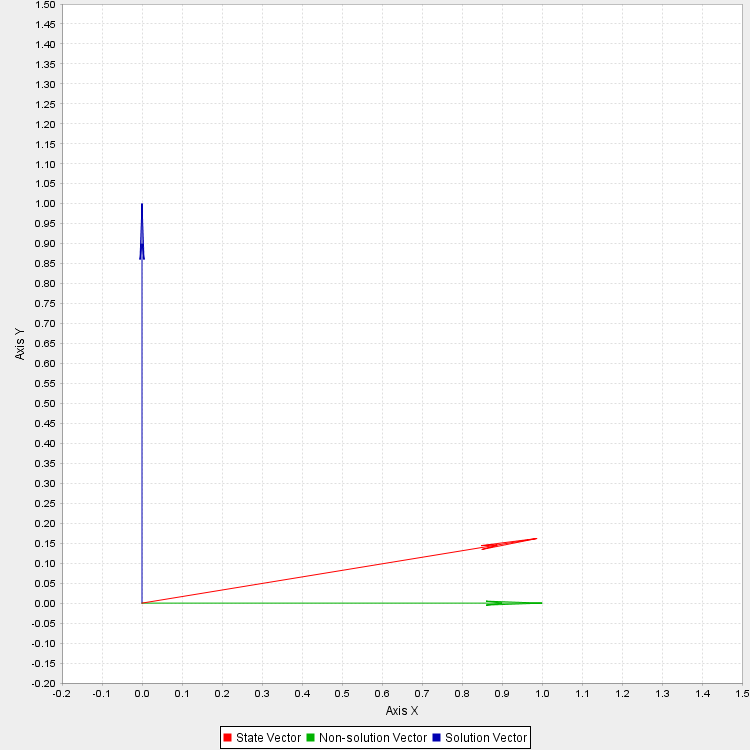
\includegraphics[width=\textwidth]{img/pic_0.png}
		\subcaption{Iteration 1 (start)}
	\end{minipage}
	\begin{minipage}{0.33\textwidth}
		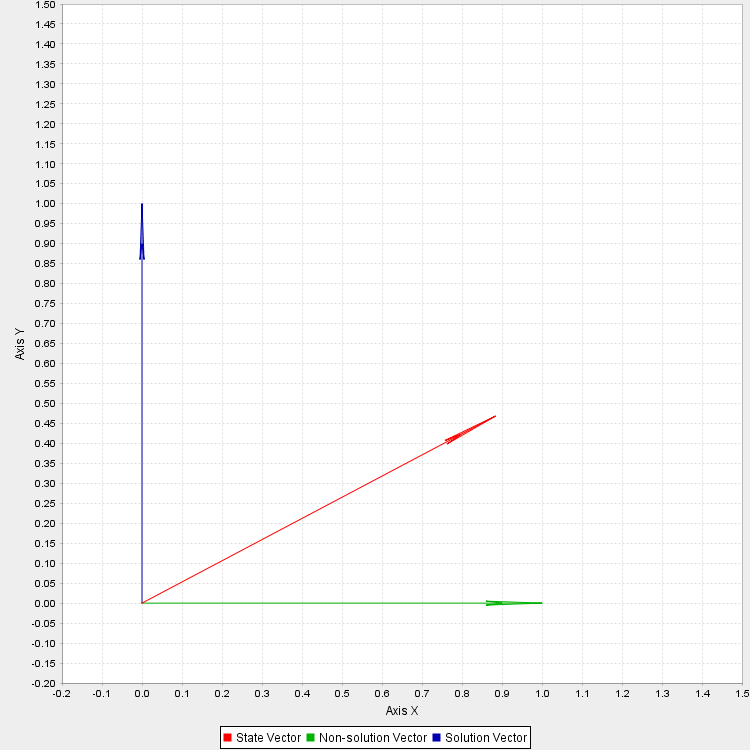
\includegraphics[width=\textwidth]{img/pic_3.png}
		\subcaption{Iteration 4}
	\end{minipage}
	\begin{minipage}{0.33\textwidth}
		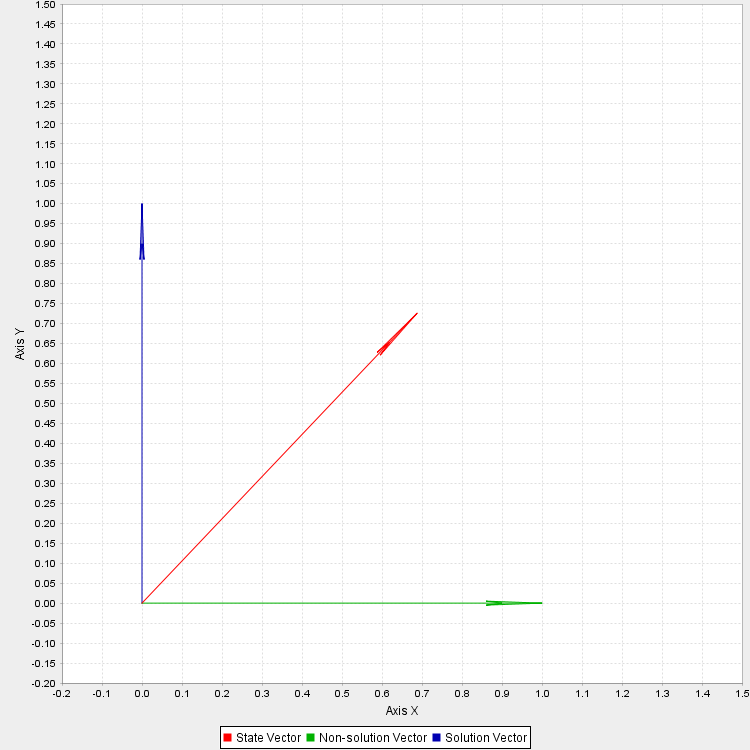
\includegraphics[width=\textwidth]{img/pic_6.png}
		\subcaption{Iteration 7}
	\end{minipage}\\
	\begin{minipage}{0.33\textwidth}
		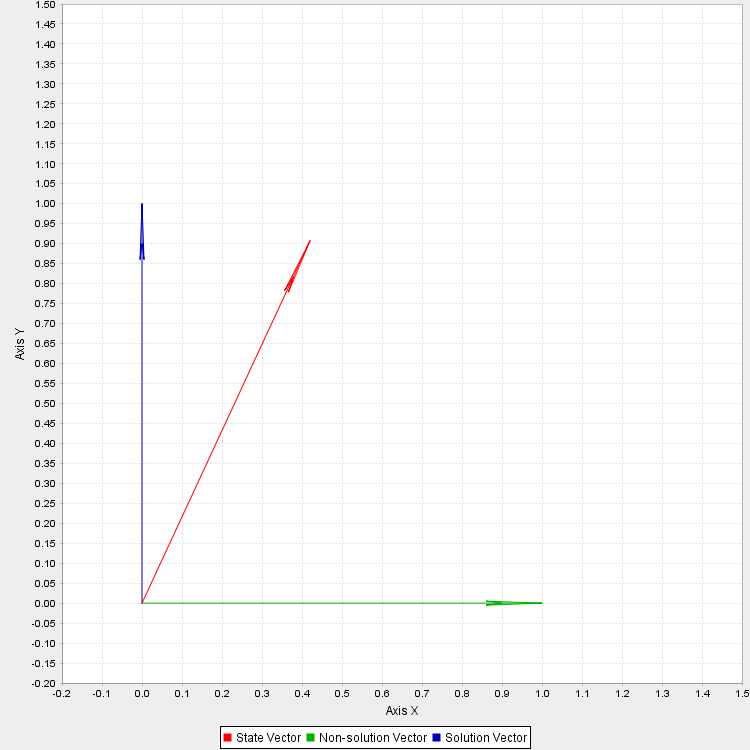
\includegraphics[width=\textwidth]{img/pic_9.png}
		\subcaption{Iteration 10}
	\end{minipage}
	\begin{minipage}{0.33\textwidth}
		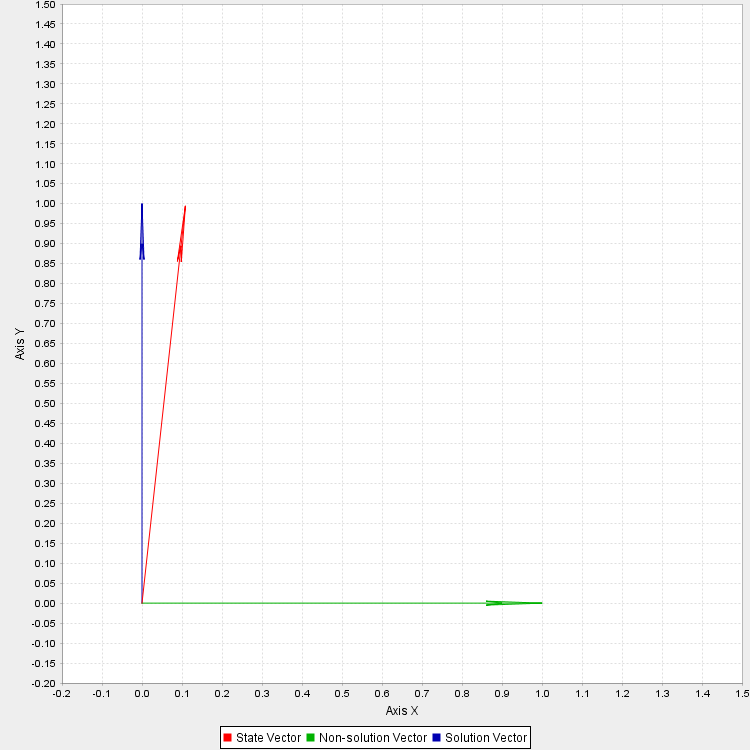
\includegraphics[width=\textwidth]{img/pic_12.png}
		\subcaption{Iteration 13}
	\end{minipage}
	\begin{minipage}{0.33\textwidth}
		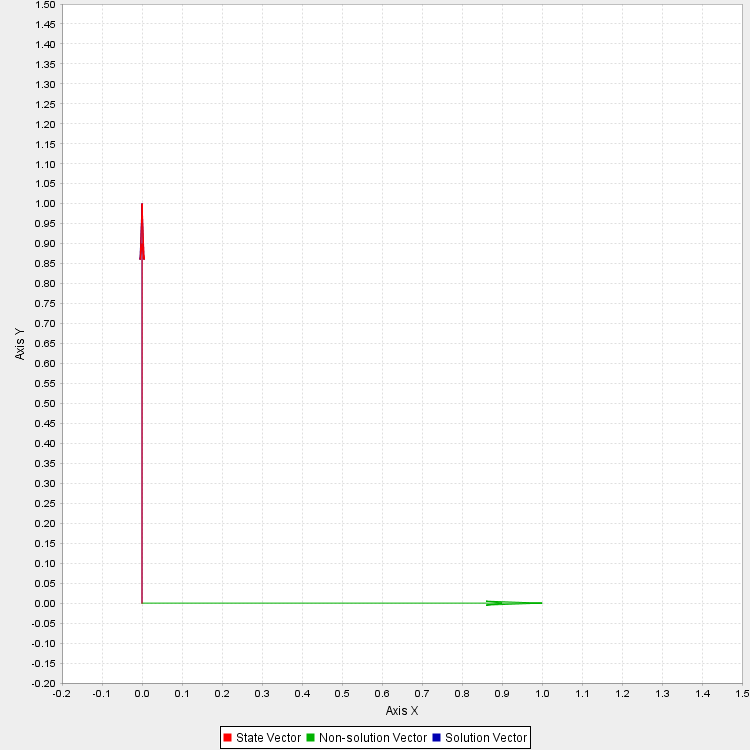
\includegraphics[width=\textwidth]{img/pic_13.png}
		\subcaption{Iteration 14 (end)}
	\end{minipage}
	\caption{Depiction of Grover's Algorithm: The green vector depicts the non-solution vector, the blue vector depicts the vector of the solution. The red vector is the projection of the current state. With every consecutive iteration the state vector rotates towards the solution state.}
	\label{grover_rotation}
\end{figure}

\subsubsection{Computational time}

Fig.\,\ref{grover_time_performance} shows the computational time of Grover's algorithm. All the measurements were executed on the same computer by varying the number of qubits $n$ for the three different representations.

We note the following observations:
\begin{itemize}
	\item\textbf{Dense representation at a disadvantage}\\
	One can see that the dense representation is the slowest one since for already $n\geq 10$ first noticeable computation times occur whereas the algorithm using functional and spare representation is still immediately executed. However, when they start to show noticeable computational times, the dense representation already takes a unbearable amount of time.
	\item\textbf{Spare vs. functional representation}\\
	Considering computational time the sparse representation is superior to the functional representation. It appears to be roughly a factor 2, but since we don't have data for bigger registers, this quantitative observation is quite vague.
	\item\textbf{Exponential behaviour}\\
	All three representations show an exponential behaviour. To illustrate the point we plotted the same data in a log-plot (Fig.\,\ref{grover_time_performance_log}) and got a linear relation.
\end{itemize}

\begin{figure}[H]
	\centering
	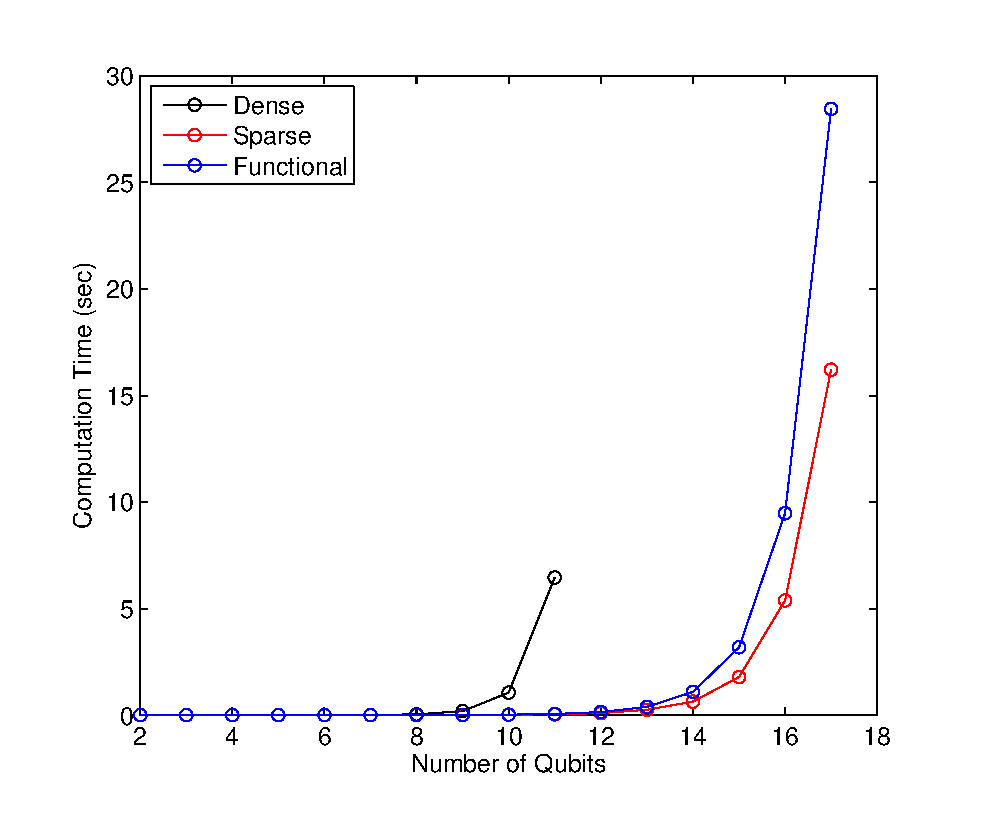
\includegraphics[width=0.9\textwidth]{img/Grover_Time_Performance.eps}
	\caption{Computational time of Grover's Algorithm in nanoseconds as a function of the quantum register size for the three different forms of representation (dense, sparse, functional).}
	\label{grover_time_performance}
\end{figure}




\subsection{Shor's Algorithm}\label{sec:Shor}


%-----------------------------------------------------------------------------------------
% DISCUSSION
%-----------------------------------------------------------------------------------------
%
\section{Discussion}\label{sec:Discussion}

\subsection{Matrix or functional representation}

\subsection{Improvements and further steps}

%-----------------------------------------------------------------------------------------
% CONCLUSION
%-----------------------------------------------------------------------------------------
%
\section{Conclusion}


%-----------------------------------------------------------------------------------------
% APPENDIX
%-----------------------------------------------------------------------------------------
%
\section{Appendix}

\subsection{Grover's Algorithm}

\begin{figure}[H]
	\centering
	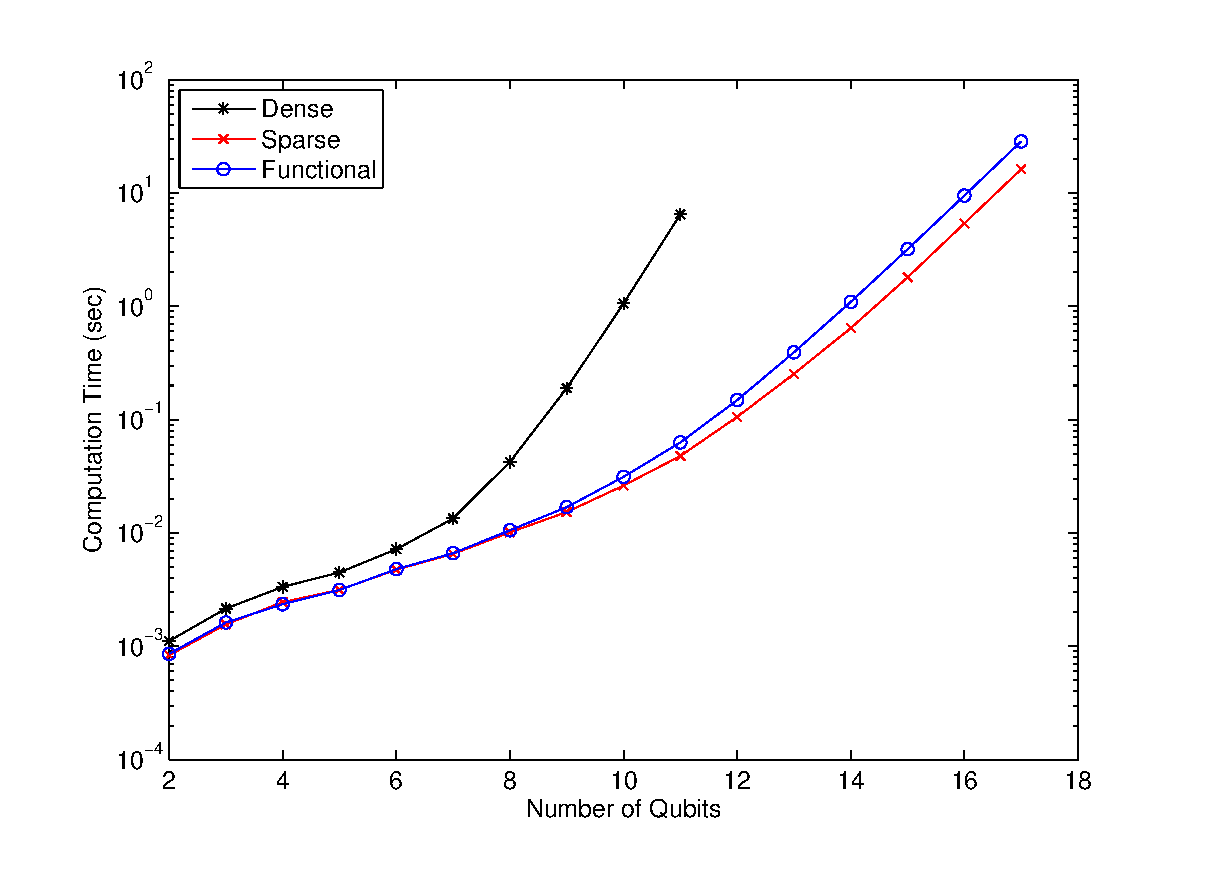
\includegraphics[width=0.9\textwidth]{img/Grover_Time_Performance_log.eps}
	\caption{Computational time (log-scale) of Grover's Algorithm in nanoseconds as a function of the quantum register size for the three different forms of representation (dense, sparse, functional). Note that only the behaviour for bigger registers is meaningful (linear).}
	\label{grover_time_performance_log}
\end{figure}

\subsection{Details}
The data for the computational time (Fig.\,\ref{grover_time_performance} and Fig.\,\ref{grover_time_performance_log}) was collected on a:

\begin{quotation}
	Intel i5 3570@3.4\,GHz\quad\quad 2x4\,GB 1600\,Mhz Ram \quad\quad Windows 7
\end{quotation}

	


%

\newpage

\phantomsection
\addcontentsline{toc}{section}{References}

\nocite{Perry2012}
\nocite{BasicConceptsQC}

\phantomsection\label{sec:References}
\bibliographystyle{plaindin}
\bibliography{lit}


\end{document}